\chapter{Related Work}


\section{Graph Theory Basics}

In this section some graph theory related notation is defined which is used during this thesis.
It is for the most part based on \cite{Thulasiraman1992} and on \cite{Diestel2012}.
A graph is a mathematical construct that can be used to model and explore the relationship between objects. 
More formally, a graph is a ordered pair of finite sets \(G = (V, E)\), whereas \(V\) denotes the set of \emph{vertices} (i.e., the objects) and \(E \subseteq [V]^2 \) the set of \emph{edges} (i.e., the relationships between the objects).
It is common to write \(V(G)\) and \(E(G)\) to refer to the set of vertices, respectively the set of edges, that are associated with a graph \(G\).
An edge \(\{v_1, v_2\} \in E(G)\) is an unordered pair of two vertices.
This means that there is no distinction between the two edges \(\{v_1, v_2 \}\) and \(\{v_2, v_1\}\). 
A graph with this property is called a \emph{undirected} graph.
However, it is also possible to define edges as ordered pairs, so that each edge does have a start- and endpoint. 
Such a graph is called a \emph{directed} graph.
An edge of the form \(\{v_i, v_i\} \in E(G)\) is called a \emph{self-loop} of the vertex \(v_i\).
Furthermore, it is possible that two distinct vertices are joined by multiple edges. 
Such edges are referred to as \emph{parallel} edges.
A graph that has no parallel edges and no self-loops is called a \emph{simple} graph.
Figure \ref{fig:example_graphs} depicts a example for a simple graph and for a graph with multiple edges and a self-loop vertex.
All further mentions and definitions for graphs are referring to undirected simple graphs unless stated otherwise.

\begin{figure}[h]
   \centering
   \begin{subfigure}[t]{0.45\textwidth}
     \centering
     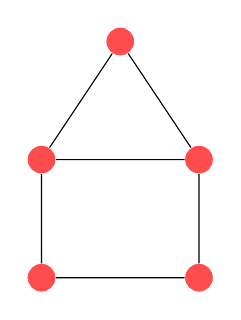
\begin{tikzpicture}[node/.style={circle,fill=red!70,minimum size=1em,inner sep=3pt]}]
       \node[node] (1) at (0, 0) {};
       \node[node] (2) at (-1, -1.5)  {};
       \node[node] (3) at (1, -1.5) {};
       \node[node] (4) at (-1, -3) {};
       \node[node] (5) at (1, -3) {};
       
       \draw (1) -- (3);
       \draw (1) -- (2) -- (4) -- (5) -- (3) -- (2);
     \end{tikzpicture}
     \caption{A undirected simple graph.}   
   \end{subfigure}
   ~
   \begin{subfigure}[t]{0.45\textwidth}
     \centering
     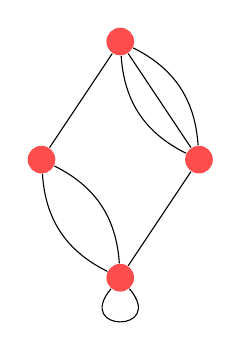
\begin{tikzpicture}[every loop/.style={}, node/.style={circle,fill=red!70,minimum size=1em,inner sep=3pt]}]
       \node[node] (1) at (0, 0) {};
       \node[node] (2) at (-1, -1.5)  {};
       \node[node] (3) at (1, -1.5) {};
       \node[node] (4) at (0, -3) {};
      
       \draw (1) -- (2);
       \draw (1) -- (3) -- (4);
       \path (2) edge [bend left] (4);
       \path (2) edge [bend right] (4);
       \path (3) edge [bend left] (1);
       \path (3) edge [bend right] (1);
       \draw (4) edge [in=-50,out=-130,loop] (4);
     \end{tikzpicture}
     \caption{A undirected graph with a self-loop and parallel edges.}
   \end{subfigure}
   
   \caption{Graphical representation of two graphs with different properties. 
   The vertices are represented by red dots and the edges are the line segments between them.} 
   \label{fig:example_graphs}
\end{figure}


The \emph{order} of a graph is its number of vertices (i.e., the cardinality of the vertex set) and is denoted as \(n = |V(G)|\). 
The neighborhood of a vertex \(v_i\) is defined as \(N(v_i) = \{v_j \in V(G) : \{v_i, v_j \} \in E(G)\}\).
It is the set of vertices that are \emph{adjacent} to the vertex \(v_i\). 
The cardinality of this set is called the \emph{degree} of the vertex and is denoted as \(d(v_i) = |N(v_i)|\). 
A vertex without any neighbors (i.e., with a degree of zero) is called \emph{isolated}.
It is also often very useful to measure degree properties for the graph. 
For example, the \emph{minimum degree} \(\delta(G) = \min\{d(v_i) : v_i \in V(G)\}\), the \emph{maximal degree} \(\Delta(G) = \max\{d(v_i) : v_i \in V(G)\}\), and the \emph{average degree} \(d(G) = \frac{1}{n} \sum_{v_i \in V(G)} d(v_i)\).
These global measures can be used to get an insight in the basic structure of the graph.

A \emph{path} on a graph can be defined as a finite sequence of vertices \(v_1,v_2,\dots,v_k\), such that between any consecutive pair of vertices exist a edge in the graph.  
Furthermore, all edges between the vertices and the vertices itself must be distinct. 
The first and the last vertices in the sequence are called the \emph{end vertices} or \emph{terminal vertices} of the path.
The \emph{path length} is the number of edges on the path.
Two vertices are \emph{connected} if it is possible to find a path with these two vertices as end points.
A vertex is, by definition, connected to itself.
If there exists a path between all pairs of vertices, then the graph is called connected.
It is possible to partition the vertex and edge set of a not connected graph in such a way that there are no edges between vertices in different partitions.
These partitions are called the \emph{components} of the graph.

The \emph{clustering coefficient} \cite{Watts1998} of a vertex is a measure for the cliquishness of its neighborhood.
A \emph{clique} in a graph is a subset of vertices, such that there exists an edge between every pair of vertices in this set.
The clustering coefficient \(C(v_i)\) is defined as the fraction of possible edges between the neighbors of the vertex \(v_i\).
There are at most \(\binom{d(v_i)}{2} = \frac{d(v_i)(d(v_i) - 1)}{2}\) possible edges between vertices in the neighborhood.
Therefore, the clustering coefficient can be calculated using the following formula.

\[ C(v_i) =  \frac{2 \, |\{\{v_j, v_k\} \in E(G) : v_j \in N(v_i) \wedge v_k \in N(v_i)\}| }{d(v_i)(d(v_i) - 1)}\]

This is, of course, a local property of one vertex.
However, it is also often useful to consider the average clustering coefficient \(C = \frac{1}{n} \sum_{v(i) \in V(G)} C(v_i)\) of the graph.
Figure \ref{fig:clustering-coefficent-examples} shows some examples for different clustering coefficients.


\begin{figure}[h]
   \centering
   \begin{subfigure}[t]{0.31\textwidth}
     \centering
     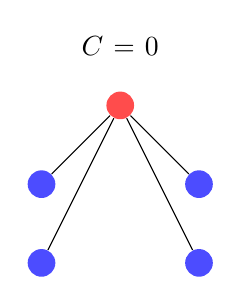
\begin{tikzpicture}[node/.style={circle,fill=red!70,minimum size=1em,inner sep=3pt]}, neighbor/.style={circle,fill=blue!70,minimum size=1em,inner sep=3pt]}]
       \node[text width=4em, align=center] at (0, 0.75)  {\(C = 0\)};
       \node[node] (1) at (0, 0) {};
       \node[neighbor] (2) at (-1, -1)  {};
       \node[neighbor] (3) at (1, -1) {};
       \node[neighbor] (4) at (-1, -2)  {};
       \node[neighbor] (5) at (1, -2) {};
       
       \foreach \p in {2,3,4,5}{\draw (\p) -- (1); }
     \end{tikzpicture}
     \caption{In this example none of the four neighbors shares a edge with any other neighbor of the red vertex.
     Therefore, the clustering coefficient of the red vertex is \(\frac{0}{6} = 0\).}   
   \end{subfigure}
   ~
   \begin{subfigure}[t]{0.31\textwidth}
     \centering
     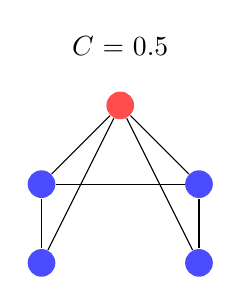
\begin{tikzpicture}[node/.style={circle,fill=red!70,minimum size=1em,inner sep=3pt]}, neighbor/.style={circle,fill=blue!70,minimum size=1em,inner sep=3pt]}]
       \node[text width=4em, align=center] at (0, 0.75)  {\(C = 0.5\)};
       \node[node] (1) at (0, 0) {};
       \node[neighbor] (2) at (-1, -1)  {};
       \node[neighbor] (3) at (1, -1) {};
       \node[neighbor] (4) at (-1, -2)  {};
       \node[neighbor] (5) at (1, -2) {};
       
       \foreach \p in {2,3,4,5}{\draw (\p) -- (1); }
       \draw (2) -- (4);
       \draw (3) -- (5);
       \draw (3) -- (2);
     \end{tikzpicture}
     \caption{Here are half of the possible edges between the neighbors are present.
     The clustering coefficient of the red vertex is \(\frac{3}{6} = \frac{1}{2}\).}
   \end{subfigure}
   ~
   \begin{subfigure}[t]{0.31\textwidth}
     \centering
     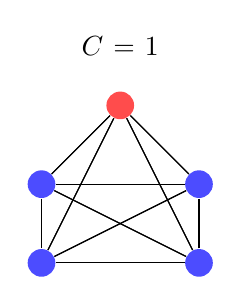
\begin{tikzpicture}[node/.style={circle,fill=red!70,minimum size=1em,inner sep=3pt]}, neighbor/.style={circle,fill=blue!70,minimum size=1em,inner sep=3pt]}]
       \node[text width=4em, align=center] at (0, 0.75)  {\(C = 1\)};
       \node[node] (1) at (0, 0) {};
       \node[neighbor] (2) at (-1, -1)  {};
       \node[neighbor] (3) at (1, -1) {};
       \node[neighbor] (4) at (-1, -2)  {};
       \node[neighbor] (5) at (1, -2) {};
       
       \foreach \p in {1,2,3,4,5}{ \foreach \q in {1,2,3,4,5}{\draw (\p) -- (\q); }}
     \end{tikzpicture}
     \caption{The neighbors of the red vertex form a clique in this example. 
     Hence, the clustering coefficient is \(\frac{6}{6} = 1\).}   
   \end{subfigure}
   
   \caption{Examples for the clustering coefficient of a vertex with a small neighborhood. 
   The blue vertices are the neighbors of the red vertex. 
   The possible number of edges between the four neighbors is \(\binom{4}{2} = 6\).} 
   \label{fig:clustering-coefficent-examples}
\end{figure}


\section{Networks and their Applications}

In the real world it is common to use graphs to model the complex systems that are arising. 
For example, the web can be represented as a graph, where the vertices correspond to websites and the edges are the hyperlinks between them. 
Another example would be a large online social networks such as Facebook, where the vertices represent the users and edges the friendship relation between them.
However, when modeling these large networks it usually common to use a slightly different terminology \cite{Barabasi2016}.
Vertices are often called \emph{nodes} and edges are called \emph{links} in the context of networks.

% TODO: large graphs = networks and network science is the statistical analysis of networks

